  \subsection{Hard Ant}
    \subsubsection{Definición}
      \paragraph{Hard Ant es uno de los bloques funcionales base de Ambienta2MX, su función principal es la de enrutar las peticiones a las bases de tipo MX además de brindar la solución cartográfica (a nivel ubicación) interactuando con Fast Eagle.}
      \paragraph{Como complemento a la arquitectura, también contará con el proceso del registro masivo de información, exponiendo servicios que el módulo Smart Owl usará de forma constante para persistir la información estandarizada de diversas fuentes de información.}
      \paragraph{Hard Ant brindará los canales de acceso a las bases MX definidas en el diagrama general mediante servicios HTTP, estos servicios brindarán información para el proceso de inserción y extracción de la información. }
      \paragraph{Este módulo es lo que sería considerado la capa del modelo de datos en un patrón MVC, ya que es la que tiene contacto de forma directa con los datos almacenados en las bases de datos orientadas a documentos gestionadas por Mongo.}
      \paragraph{Se utilizará un pool de conexiones a la base para garantizar el acceso o escritura a los datos además de brindar la posibilidad de respuestas asincronas y no bloqueantes entre las consultas realizadas.}
      \paragraph{Considerando trabajos más pesados (Obtención de datos históricos) se utilizarán procesos en segundo plano, esto es posible gracias a la implementación de ``Verticles'' nativas de Vert.x, tecnología que será usada para el desarrollo y despliegue final de éste módulo.}
      \newpage
        \begin{landscape}
          \subsubsection{Diagrama por bloques}
          \paragraph{A continuación se mostrará el diagrama por bloques que define la estructura de Hard Ant.}
          \begin{figure}[b!]
          \centering
          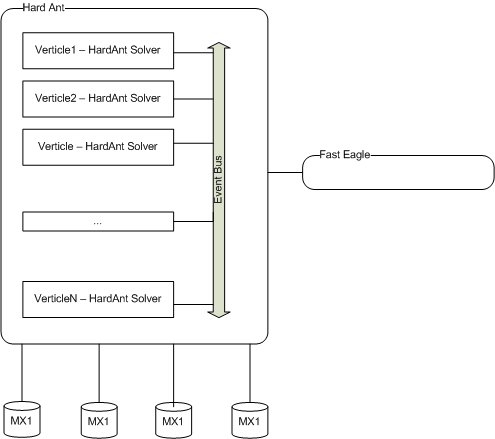
\includegraphics[width=17.5cm,height=12cm]{./images/DiagramaHardAnt.png}
          \caption{Diagrama General de Hard Ant}
        \end{figure}
        \end{landscape}
      \newpage
    \paragraph{En el diagrama se puede apreciar la replicación de ``Verticles'' que interactuan a través del mismo canal de información, esto brinda una alta disponibilidad del servicio ya que las peticiones son atendidas y procesadas no sólo por un elemento existente si no varios. Otros módulos de Ambienta2MX pueden conectarse a este canal de información ya sea de forma local o distribuida.}